\ifx\mlbook\undefined
    \documentclass[10pt,a4paper]{ctexbook}
    \providecommand{\pathroot}{../..}

    \usepackage[CJKbookmarks,colorlinks,linkcolor=red]{hyperref}
    \usepackage{geometry}
    \usepackage{amsmath}
    \usepackage{minted}

    \geometry{left=3.0cm,right=3.0cm,top=2.5cm,bottom=2.5cm}
    \setmainfont{SimSun}
    \XeTeXlinebreaklocale "zh"
    \XeTeXlinebreakskip = 0pt plus 1pt minus 0.1pt

    \begin{document}
    \setlength{\baselineskip}{20pt}
    \title{Logistic回归}
    \author{Donald Cheung\\jianzhang9102@gmail.com}
    \date{Sep 8, 2017}
    %\maketitle
    \tableofcontents
\fi

\chapter{Logistic Regression}
这一章用来介绍常用的线性模型,主要包括:多元线性回归、Logistic回归(LR)。

\href{http://www.cs.cmu.edu/~sgopal1/papers/ICML13.pdf}{Distributed Training of Large-scale Logistic models}

\section{sigmoid函数}
sigmoid函数是常用的数学函数之一,它的数学表达式为
\[
    h_{\theta}(x)=g({\theta}^Tx)={\frac {1}{1+e^{-\theta^Tx}}}
\]
数学图像如图\ref{fig:sigmoid}所示。

\begin{figure}[ht]
    \centering
    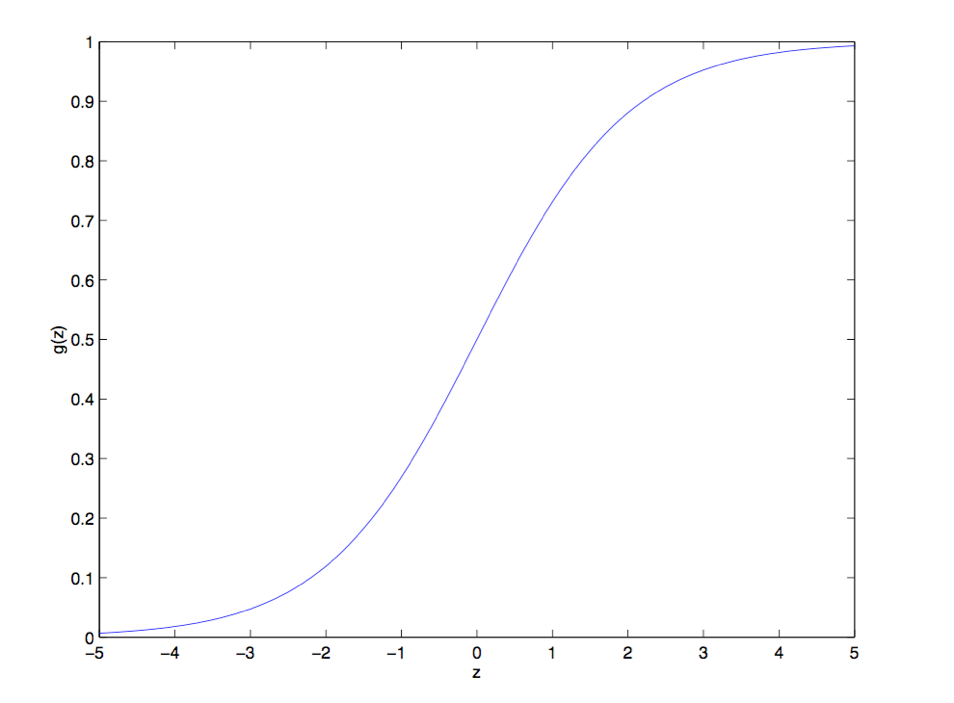
\includegraphics[height=7cm]{\pathroot/theory/GLM/images/sigmoid.png}
    \caption{sigmoid函数}
    \label{fig:sigmoid}
\end{figure}

函数可导:
\[
g'(z)={\frac {d}{dz}}{\frac {1}{1+e^{-\theta^Tx}}}=\lim_{{\Delta x}\to 0}{\frac {f(x+{\Delta x})-f(x)}{\Delta x}}
\]

对于一个二分类问题,可假设$h_{\theta}(x)$为其中一类的概率,即:
\[
P(y=1|x;\theta)=h_{\theta}(x)
               =h_{\theta}(x)^{1}(1-h_{\theta}(x))^{1-1}
               =h_{\theta}(x)^{y}(1-h_{\theta}(x))^{1-y}
\]

\[
P(y=0|x;\theta)=1-h_{\theta}(x)
               =h_{\theta}(x)^{0}(1-h_{\theta}(x))^{1-0}
               =h_{\theta}(x)^{y}(1-h_{\theta}(x))^{1-y}
\]


\begin{minted}[mathescape,
               numbersep=5pt,
               frame=lines,
               framesep=2mm]{python}
class SimpleLogisticRegression(object):
    def __init__(self, alpha, feature_num):
        pass
    def fit(self, X, y, verbose=False):
        last_target = -sys.maxint
        last_step = 0
        step = 0
        while True:
            step += 1
            # 计算梯度并更新参数
            target = sum(map(lambda py, ty: ty * math.log(py) + (1 - ty) * math.log(1 - py),
                             map(self.__sigmoid, X), y)) / len(X)
            if target - last_target > 1e-8:
                last_target = target
                last_step = step
            elif step - last_step >= 10:
                break
        target = sum(map(lambda py, ty: ty * math.log(py) + (1 - ty) * math.log(1 - py),
                         map(self.__sigmoid, X), y)) / len(X)
        return target


    def predict(self, X):
        pass
    def __sigmoid(self, x):
        pass
    def _check_columns(self, X):
        pass

if __name__ == "__main__":
    lr = SimpleLogisticRegression(0.1, 3)
    X = [[1, 3, 5], [2, 4, 6], [3, 5, 7], [4,  6, 8]]
    y = [0, 0, 1, 1]
    print lr.predict(X)
    lr.fit(X, y, verbose=True)
    print lr.predict(X)
\end{minted}

\begin{minted}[mathescape,
               numbersep=5pt,
               frame=lines,
               framesep=2mm]{python}
#coding: utf-8
#author: Ryan
from __future__ import division
import sys
import os
import random
import math
import collections
import array
import operator

class SimpleLogisticRegression(object):
    def __init__(self, alpha, feature_num):
        """构造函数
        参数
        ---
        alpha: double
            学习率
        feature_num: int
            特征数量
        """
        self.__alpha = alpha
        self.__features_num = feature_num
        self.__coef = [0.] * self.__features_num
        self.__intercept = 0.

    def fit(self, X, y, verbose=False):
        """训练模型。
        返回值
        ------
            模型训练的最终log似然值。
        """
        last_target = -sys.maxint
        last_step = 0
        step = 0
        while True:
            step += 1
            gradient = [0.] * (self.__features_num + 1)
            for tx, ty in zip(X, y):
                delta = ty - self.__sigmoid(tx)
                for i, xi in enumerate(tx):
                    gradient[i] += delta * xi
                gradient[-1] += delta
            gradient = map(lambda g: g / len(X), gradient)

            self.__coef = map(lambda c, g: c + self.__alpha * g, self.__coef, gradient[:-1])
            self.__intercept += self.__alpha * gradient[-1]

            target = sum(map(lambda py, ty: ty * math.log(py) + (1 - ty) * math.log(1 - py),
                             map(self.__sigmoid, X), y)) / len(X)
            if target - last_target > 1e-8:
                last_target = target
                last_step = step
            elif step - last_step >= 10:
                break
            if verbose is True and step % 1000 == 0:
                sys.stderr.write("step %s: %.6f\n" % (step, target))
        target = sum(map(lambda py, ty: ty * math.log(py) + (1 - ty) * math.log(1 - py),
                         map(self.__sigmoid, X), y)) / len(X)
        if verbose is True:
            sys.stderr.write("Final training error: %.6f\n" % (target))
        return target

    def predict(self, X):
        """输出每个样本的预测值。
        返回值
        -----
            列表类型,长度与X的样本量相同。
        """
        if not self._check_columns(X):
            sys.stderr.write("The data to be evaluated can't match training data's features\n")
            return None
        return map(self.__sigmoid, X)

    def __sigmoid(self, x):
        """sigmoid函数,返回sigmoid函数值"""
        return 1. / (1 + math.exp(-sum(map(operator.mul, self.__coef, x)) - self.__intercept))

    def _check_columns(self, X):
        """检查每个样本的类型是否是数组或者列表类型,并且长度与特征数相等。
        返回值
        -----
            数据合法时,返回True,否则返回False。
        """
        for x in X:
            if not isinstance(x, (list, tuple, array.array)):
                return False
            if len(x) != self.__features_num:
                return False
        return True

if __name__ == "__main__":
    lr = SimpleLogisticRegression(0.1, 3)
    X = [[1, 3, 5], [2, 4, 6], [3, 5, 7], [4,  6, 8]]
    y = [0, 0, 1, 1]
    print lr.predict(X)
    lr.fit(X, y, verbose=True)
    print lr.predict(X)
\end{minted}


\begin{itemize}
\item 更简洁的形式: $P(y|x;\theta)={h_{\theta}(x)}^y(1-h_{\theta}(x))^{1-y}$
\item 假设$m$个训练样本独立,则样本集在参数${\theta}$给定下,出现的概率为
\begin{align*}
L(\theta)&=p(\vec y|X;\theta)\\
         &=\prod_{i=1}^{m}{p(y^{(i)} | x^{(i)};\theta)}\\
         &=\prod_{i=1}^{m}{(h_{\theta}(x^{(i)}))^{y^{(i)}}(1-h_{\theta}(x^{(i)}))^{(1-y^{(i)})}}
\end{align*}

\item 我们希望最大化概率$L({\theta})$,也即最大化log似然值:

\item 最大化一个目标值,可采用梯度上升法,沿着梯度方向不断迭代。梯度求解如下:

\item 随机梯度下降法求解:
\subitem ${\theta}_{j}:={\theta}_{j}+{\alpha}(y^{(i)}-h_{\theta}(x^{(i)}))x_{j}^{(i)}$

\item 思考:
\subitem 如果引入$L1$正则、$L2$正则,那么梯度又该怎么求解呢?
\subitem LR的梯度求解公式与线性回归的梯度求解公式看起来一样,有区别么?

\item L1:$cost(w)={\frac {1}{2m}}\left\|{Xw-y}\right\|^{2}+\lambda\|w\|_{1}$
,等价于
    $\min\limits_{w}{\frac {1}{2m}}\left\|{Xw-y}\right\|^{2}, s.t. \left\|w\right\|_{1}\le{C}$

\item L2:$cost(w)={\frac {1}{2m}}\left\|{Xw-y}\right\|^{2}+{\frac {\lambda}{2}}\|w\|_{2}^{2}$
,等价于
    $\min\limits_{w}{\frac {1}{2m}}\left\|{Xw-y}\right\|^{2}, s.t. \left\|w\right\|_{2}^{2}\le{C}$

\item 常用分类器的评价指标有:准确率(precision)、召回率(recall)、F值、正确率(accuracy)等
\end{itemize}

\begin{itemize}

\item 考虑ROC曲线图中的四个点。
    \subitem(1)第一个点(0,1),FPR=0, TPR=1,即FN=0,并且FP=0。
        \subsubitem 特点:正确分类所有的样本。
    \subitem(2)第二个点(1,0),FPR=1,TPR=0。
        \subsubitem 特点:成功错分了所有的样例。
    \subitem(3)第三个点(0,0),FPR=TPR=0,即FP=TP=0,
        \subsubitem 特点:分类器预测所有的样本都为负样本。
    \subitem(4)第四个点(1,1),分类器预测所有的样本都为正样本。
\item 结论:ROC曲线越接近左上角,该分类器的性能越好。
\item 考虑ROC曲线图中的虚线$y=x$上的点。这条对角线上的点表示的是一个采用随机猜测策略的分类器的结果。

\item ROC曲线的画法:对一个特定的测试数据集合,对分类模型输出的概率值设置不同的阈值,从而得到一组(FPR,TPR)点,以此连接这些点即可得到ROC曲线。
\item AUC(Area Under Curve):ROC曲线下的面积。
\item AUC值等于一个随机选择的正样本的预测值高于一个随机选择的负样本的概率。
\item ROC曲线的优点:当测试集中的正负样本的分布变化的时候,ROC曲线能够保持不变。

\item 在右图中,(a)和(c)为ROC曲线,(b)和(d)为\\
Precision-Recall曲线。(a)和(b)展示的是\\
分类其在原始测试集(正负样本分布平衡)\\
的结果,(c)和(d)是将测试集中负样本的数\\
量增加到原来的10倍后, 分类器的结果。可\\
以明显的看出,ROC曲线基本保持原貌,\\
而Precision-Recall曲线则变化较大。
\end{itemize}

\section{LR解决多分类问题}
基本思路:将多分类任务拆若干个二分类任务。学习时分别训练多个分类器,测试时对这多个分类器的预测结果进行集成以获得最终的多分类结果。

一般来说,有以下几种做法。

\subsection{一对一(OvO) }
以$C_{i}$与$C_{j}$的数据作为正反例训练一个分类器,共训练${\frac {N(N-1)}{2}}$个分类器
预测时将样本提交给所有分类器,获取${\frac {N(N-1)}{2}}$个结果,最终结果通过投票产生

\subsection{一对多(OvR)}
以$C_{i}$数据为正例,其余类别数据为负例,训练$N$个分类器

\subsection{其他}
如多对多(MvM)策略的ECOC编码


\section{在线学习算法FTRL}
\href{http://www.cnblogs.com/EE-NovRain/p/3810737.html}{各大公司广泛使用的在线学习算法FTRL详解}
\href{https://zhuanlan.zhihu.com/dataman/20447450}{在线机器学习FTRL(Follow-the-regularized-Leader)算法介绍}

现在做在线学习和CTR常常会用到逻辑回归( Logistic Regression),而传统的批量(batch)算法无法有效地处理超大规模的数据集和在线数据流,google先后三年时间(2010年-2013年)从理论研究到实际工程化实现的FTRL(Follow-the-regularized-Leader)算法,在处理诸如逻辑回归之类的带非光滑正则化项(例如1范数,做模型复杂度控制和稀疏化)的凸优化问题上性能非常出色,据闻国内各大互联网公司都第一时间应用到了实际产品中,我们的系统也使用了该算法。这里对FTRL相关发展背景和工程实现的一些指导点做一些介绍,凸优化的理论细节不做详细介绍,感兴趣可以去查阅相应paper,相关paper列表会在文后附上。机器学习并非本人在校时的专业方向,不过在校期间积累的基础不算太差,而且很多东西也是相通的,钻研一下基本意思都还能搞明白。当然,有不准确的地方欢迎大家讨论指正。

本文主要会分三个部分介绍,如果对理论产生背景不感兴趣的话,可以直接看第3部分的工程实现(这一部分google13年那篇工程化的paper介绍得很详细):
\begin{enumerate}
\item 相关背景:包括通用性的问题描述、批量算法、传统在线学习算法等
\item 简单介绍与FTRL关系比较密切的Truncated Gradient、FOBOS以及RDA(Regularized Dual Averaging)等算法
\item FTRL理论公式以及工程实现(对前因后果和理论方面不感兴趣的可以直接看这一小节的工程实现部分)
\end{enumerate}


\subsection{相关背景}
\subsubsection{问题描述}
对于loss函数+正则化的结构风险最小化的优化问题(逻辑回归也是这种形式)有两种等价的描述形式,以1范数为例,分别是:
\begin{enumerate}
\item \textbf{无约束优化形式}的soft regularization formulation:
\[
\hat{w}=arg\min\limits_{w}{\sum\limits_{i=1}^{n}{L(w,z_{i})+g\left\|w\right\|_{1}}}
\]

\item \textbf{带约束项的凸优化}问题convex constraint formulation:
\[
\hat{w}=arg\min\limits_{w}{\sum\limits_{i=1}^{n}{L(w,z_{i})}}, \quad subject \quad to \left\|w\right\|_{1} \le s
\]

\end{enumerate}
当合理地选择$g$时,二者是等价的。这里提这两种形式的问题描述,原因在于引出下面无约束优化和带约束优化问题的不同算法,对于不同的描述形式,会有一系列相关算法。

\subsubsection{批量(batch)算法}
批量算法中每次迭代对全体训练数据集进行计算(例如计算全局梯度),优点是精度和收敛还可以,缺点是无法有效处理大数据集(此时全局梯度计算代价太大),且没法应用于数据流做在线学习。这里分无约束优化形式和约束优化(与上面问题描述可以对应起来)两方面简单介绍一下一些传统批量算法。

\begin{enumerate}
\item 无约束优化形式:
    \begin{enumerate}
    \item 全局梯度下降$x_{t+1}=x_{t}-\eta\nabla{f(x_{t})}$,很常用的算法,就不细说了,每一步求一个目标函数的全局梯度,用非增学习率进行迭代;
    \item 牛顿法(切线近似)、LBFGS(割线拟牛顿,用之前迭代结果近似Hessian矩阵的逆矩阵,BFGS似乎是几个人名的首字母的简称)等方法。牛顿和拟牛顿等方法一般对于光滑的正则约束项(例如2范数)效果很好,据说是求解2范数约束的逻辑回归类问题最好的方法,应用也比较广,但是当目标函数带L1非光滑、带不可微点的约束项后,牛顿类方法比较无力,理论上需要做修改。感兴趣的可以去查查无约束优化的相关数值计算的书,我也没有更深入研究相关细节,这里不做重点关注。
    \end{enumerate}

\item 不等式约束凸优化形式:
    \begin{enumerate}
    \item 传统的不等式约束优化算法内点法等;
    \item 投影梯度下降(约束优化表示下),$g_{t}$是subgradient,直观含义是每步迭代后,迭代结果可能位于约束集合之外,然后取该迭代结果在约束凸集合上的投影作为新的迭代结果(第二个公式中那个符号标识向X的投影):
        \begin{figure}[ht]
            \centering
            \includegraphics[height=5cm]{\pathroot/theory/GLM/images/projection_subgradient.jpg}
            \begin{align*}
            & y_{t+1}=x_{t}-\eta g_{t},\ where\ g_{t} \in \partial{f(x_{t})} \\
            & x_{t+1}=\prod_{\chi}(y_{t+1})
            \end{align*}
            \caption{投影梯度下降}
            \label{fig:projection_subgradient}
        \end{figure}
    \end{enumerate}
\end{enumerate}

\subsubsection{在线算法}
如上所述,批量算法有自身的局限性,而在线学习算法的特点是:每来一个训练样本,就用该样本产生的loss和梯度对模型迭代一次,一个一个数据地进行训练,因此可以处理大数据量训练和在线训练。常用的有在线梯度下降(OGD)和随机梯度下降(SGD)等,本质思想是对上面\textbf{问题描述}中的未加和的单个数据的loss函数$L(w, z_{i})$做梯度下降,因为每一步的方向并不是全局最优的,所以整体呈现出来的会是一个看似随机的下降路线。典型迭代公式如下:
\[
w_{t+1}=\prod_{\mathcal{C}}(w_{t}-\alpha_{t}(g_{t}+\xi_{t}))
\]

这里使用混合正则化项:$\Psi(w)=I_{\mathcal{C}}(w)+\psi(w)$,例如可能是1范数与2范数强凸项的混合$\Psi(w)=\lambda\left|w\right\|_{1}+(\sigma/2)\left\|w\right\|_{2}^{2}$(后面会看到其实很多都是这种混合正则化的格式,而且是有一定直观含义的)。迭代公式中:$g_{t}$是loss函数(单点的loss,未加和)的subgradient,与$g_{t}$相加的那一项是混合正则化项中的第二项的梯度,投影集合$\mathcal{C}$是约束空间(例如可能是1范数的约束空间),跟上面介绍的投影梯度下降类似的做法。

梯度下降类的方法的优点是精度确实不错,但是不足相关paper主要提到两点:

\begin{enumerate}
\item 简单的在线梯度下降很难产生真正稀疏的解,稀疏性在机器学习中是很看重的事情,尤其我们做工程应用,稀疏的特征会大大减少predict时的内存和复杂度。这一点其实很容易理解,说白了,即便加入L1范数(L1范数能引入稀疏解的简单示例可以产看PRML那本书的第二章,我前面一篇blog的ppt里也大概提了),因为是浮点运算,训练出的w向量也很难出现绝对的零。到这里,大家可能会想说,那还不容易,当计算出的w对应维度的值很小时,我们就强制置为零不就稀疏了么。对的,其实不少人就是这么做的,后面的Truncated Gradient和FOBOS都是类似思想的应用;

\item 对于不可微点的迭代会存在一些问题,具体有什么问题,有一篇paper是这么说的:the iterates of the subgradient method are very rarely at the points of non-differentiability。我前后看了半天也没看明白,有熟悉的同学可以指导一下。
\end{enumerate}

相关参考论文:\href{https://www.eecs.tufts.edu/~dsculley/papers/ad-click-prediction.pdf}{Ad Click Prediction: a View from the Trenches}



第二期: 知临分享Online Learning的算法和业界使用
LR问题传统的batch训练(OWLQN、CDN)
增量训练作为补充——对近期数据更多的考虑
Batch需要扫描大量数据很多遍(20~100次),耗时较大
增量训练需要扫描较多数据(几个小时),耗时相对较少
第三期: 方杰分享 Online Learning的前世今生
离线学习VS在线学习
正则化
稀疏性,精度
FOBOS
RDA
FTRL


\section{大规模离散LR}
考虑有一个离散值特征A(分别有类别A1、A2、A3)和连续值特征B,采用One-Hot的表示方式,则LR的表示形式为:
\[
h(x)=\frac{1}{1+e^{-(w_{0}A_{1}+w_{1}A_{2}+w_{2}A_{3}+w_{3}B)}}
\]

\[
h(x)=\frac{1}{1+e^{-(w_{0}A_{1}+w_{1}A_{2}+w_{2}A_{3}+w_{3}B_{1}+w_{4}B_{2}+w_{5}B_{3})}}
\]




\ifx\mlbook\undefined
    \end{document}
\fi
